\chapter{Arrays and Vectors}
\section{Arrays}
\subsection{Definition}
\textbf{What is an array?}\\
Arrays are a compound data type or data structure. In other words, they are collections of elements and all the elements are of the same type. Each element can be accessed directly.\\
But why do we need arrays?\\
Let's say as a school administrator, we are supposed to model the scores of all the students out of 100. We can try to declare them one by one seperately:

\begin{lstlisting}[language=c]
int test_score_1 {0};
int test_score_2 {0};
int test_score_3 {0};
int test_score_4 {0};
int test_score_5 {0};
.
.
int test_score_100 {0};
\end{lstlisting}
This method becomes tedious and error-prone. This is where arrays are useful.
\subsection{Characteristics}
\begin{itemize}
    \item Arrays are fixed in size.
    \item Elements are all the same type as said before.
    \item Stored contiguosuly in memory. In other words, they are stored as one chunk.
    \item Individual elements can be accessed by their position or index.
    \item First element is at index 0.
    \item Last element is at index size -1.
    \item The compiler doesn't check to see if you are out of bounds. This duty lays on the programmers hands. 
    \item They are very efficient but still not as efficient as vectors. 
    \item Iteration ( looping ) is often used to process. 
\end{itemize}

\subsection{Declaring}
Following is how arrays are declared in C++ language: 
\begin{mdframed}
\begin{lstlisting}[language=c]
Element_Type array_name [constant number of elements];
\end{lstlisting}
\end{mdframed}
Some more examples to get a better grasp of how the formatting goes:
\begin{mdframed}
\begin{lstlisting}[language=c]
int test_scores [5];

int high_score_per_level [10];

const int days_in_year {365};
double hi_temperature [days_in_year];

\end{lstlisting}
\end{mdframed}

\subsection{Initialization}
Best practice is always initialize arrays as we declare them. Syntax is similar to when we used define arrays with unknown elements. 
\begin{mdframed}
\begin{lstlisting}[language=c]
Element_Type array_name [number of elements] {init list};
\end{lstlisting}
\end{mdframed}
Some examples:
\begin{mdframed}
\begin{lstlisting}[language=c]
int test_scores [5] {100,95,99,87,88};

int high_score_per_level [10] {3,5};
// init to 3,5 and remaining to 0

const double days_in_year {365};
double hi_temperatures [days_in_year] {0};
// init all to zero

int another_array [] {1,2,3,4,5}
// size automatically calculated
\end{lstlisting}
\end{mdframed}

\subsection{Accessing Array Elements}
The syntax-ing is very much like expected:

\begin{mdframed}
\begin{lstlisting}[language=c]
array_name [element_index];
test_scores [1];
\end{lstlisting}
\end{mdframed}
\begin{mdframed}
\begin{lstlisting}[language=c]
int test_scores [5] {100,98,99,87,88};
cout << "First score: " << test_scores[0] << endl;
cout << "Second score: " << test_scores[1] << endl;
cout << "Third score: " << test_scores[2] << endl;
cout << "Fourth score: " << test_scores[3] << endl;
cout << "Fifth score: " << test_scores[4] << endl;
\end{lstlisting}
\end{mdframed}
We also use the same syntax-ing for storing values in an array's elements.
\begin{mdframed}
\begin{lstlisting}[language=c]
int test_scores [5] {100,98,99,87,88};
cin >> test_scores[0]; 
cin >> test_scores[1]; 
cin >> test_scores[2];
cin >> test_scores[3];
cin >> test_scores[4];

// assignment statement
test_scores[0] = 90;
\end{lstlisting}
\end{mdframed}
\textbf{How does it work?}\\
The name of the array represents the location of the first element in array ( index 0 ). The [index] represents the offset from the beginning of that array and finally C++ simply performs a calculation to find the correct element. However, the compiler doesn't check the bounds so it's important to remember there is no bounds checking in C++ language and the program may crash. 
\subsection{Multi-dimensional Arrays}
In order to define multi-dimensional arrays, all we have to do is add another dimension using a set of square brackets. 
\begin{mdframed}
\begin{lstlisting}[language=c]

Element_Type array_name [dim1_size] [dim2_size];
int movie_rating [3][4];

\end{lstlisting}
\end{mdframed}
We can model real-world data to show the application of n-dimensional arrays ( 2 in this case ). Suppose we want to collect movie ratings, and each reviewer has reviewed and set a score for multiple movies. To be exact, 3 reviewers have reviewed 4 movies each. 

\begin{figure}[h]
\centering
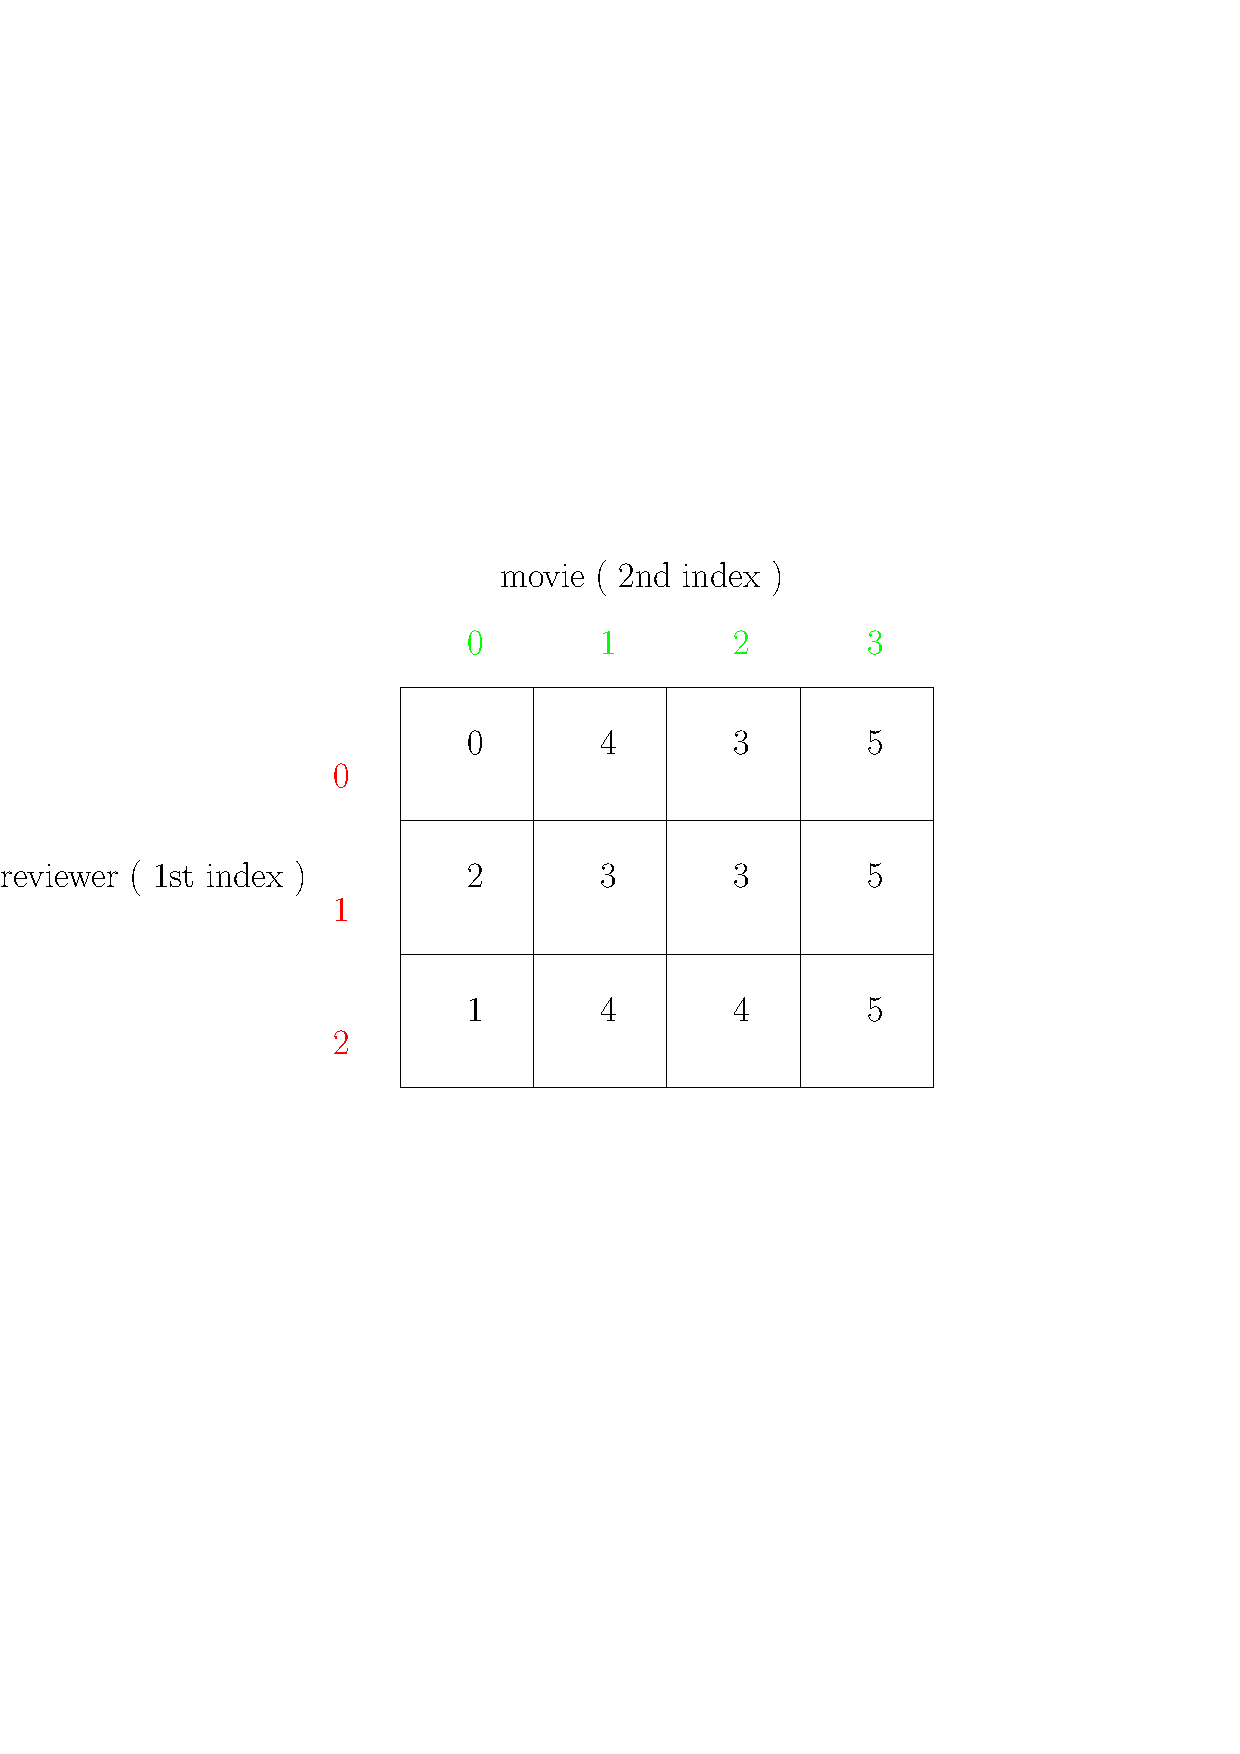
\includegraphics[width=0.70\linewidth]{1.pdf}
\caption{\label{fig:1}Rows and Columns of 2D Array}
\end{figure}

\begin{mdframed}
\begin{lstlisting}[language=c]
const int rows {3};
const int cols {4};
int movie_rating [rows] [cols];
\end{lstlisting}
\end{mdframed}
In order to access array elements in n-dimensional arrays:
\begin{mdframed}
\begin{lstlisting}[language=c]
cin >> movie_rating [1] [2];
cout << movie_rating [1] [2];
\end{lstlisting}
\end{mdframed}

\begin{figure}[h]
\centering
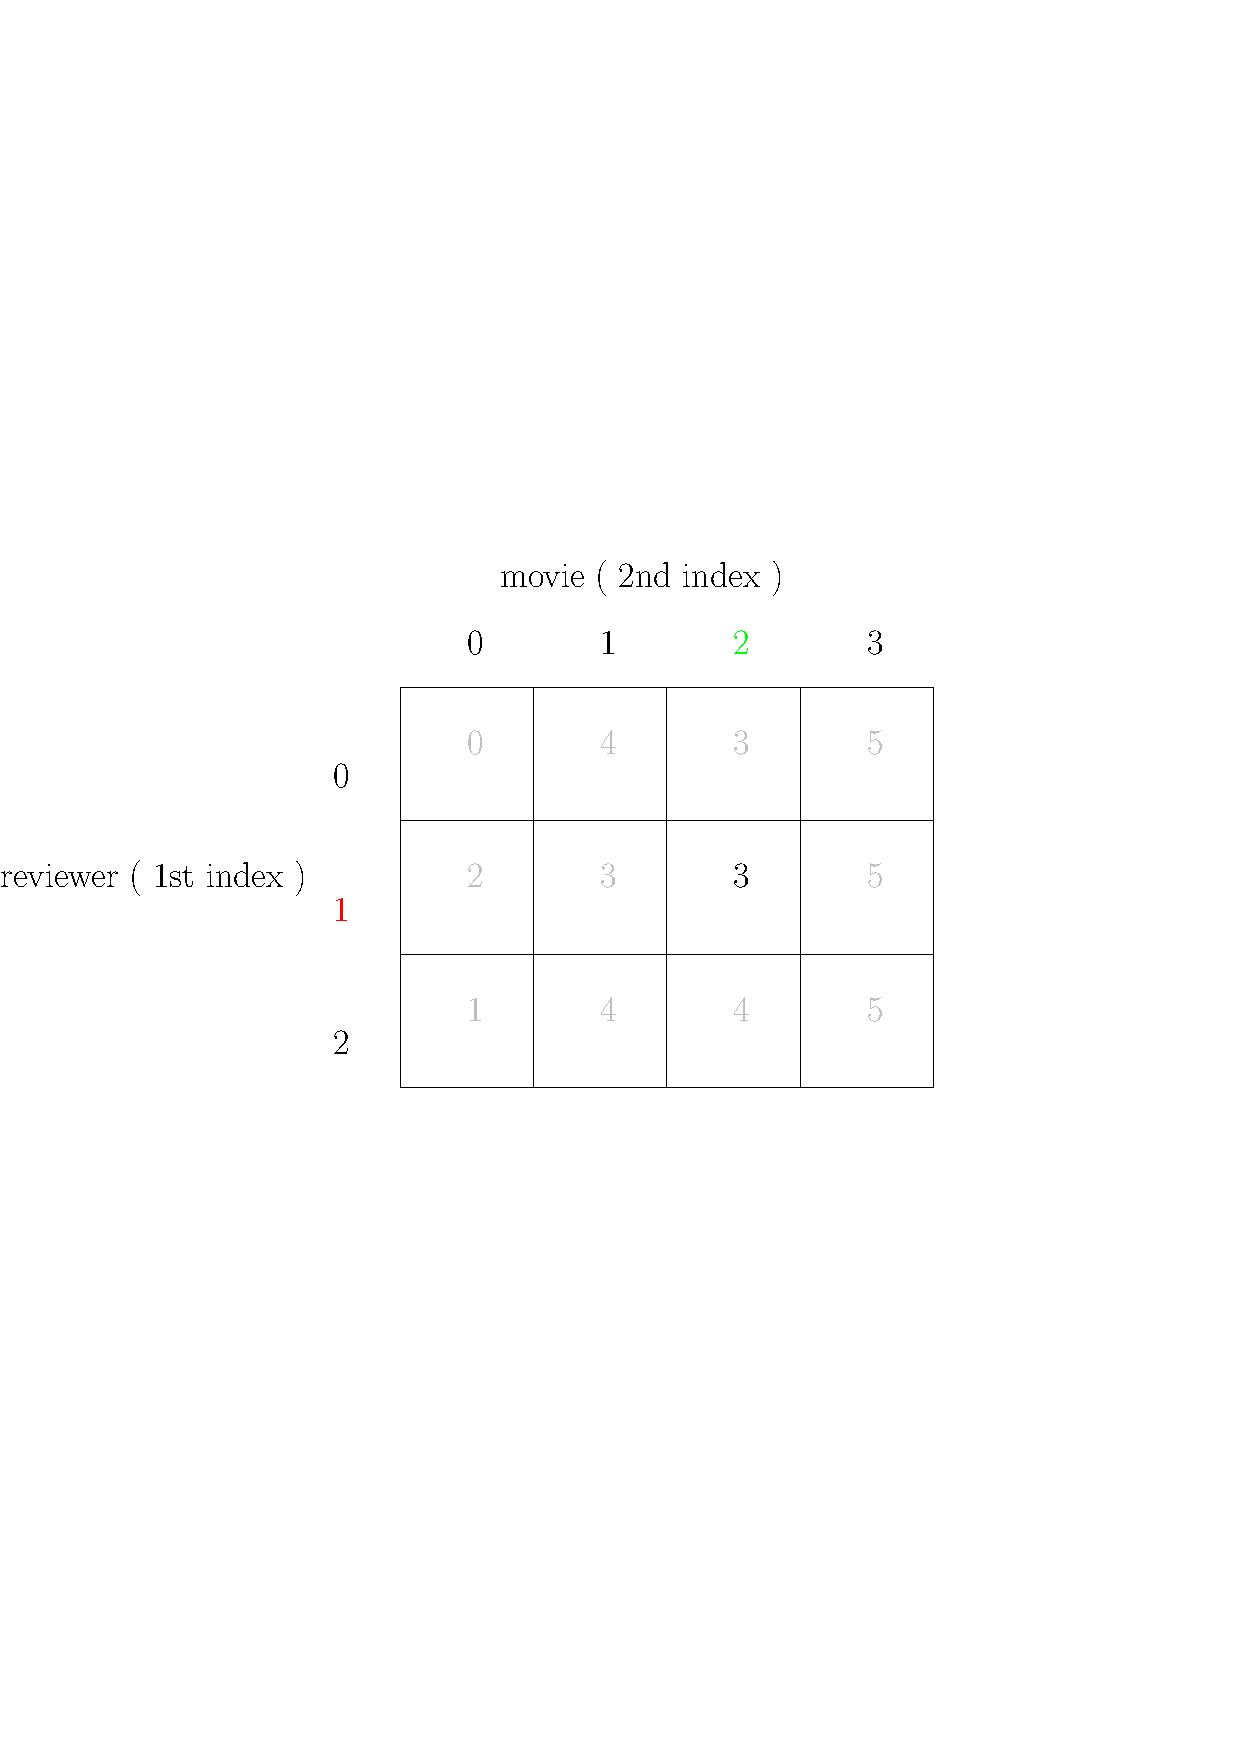
\includegraphics[width=0.70\linewidth]{2.pdf}
\caption{\label{fig:2}Rows and Columns of 2D Array}
\end{figure}
If we wanted to initialize a 2D array, we could type:
\begin{mdframed}
\begin{lstlisting}[language=c]
int movie_rating [3] [4]
{
    {0, 4, 3, 5},
    {2, 3, 3, 5},
    {1, 4, 4, 5}
};
\end{lstlisting}
\end{mdframed}
However, even though arrays can be useful, in modern C++ using vectors is always prioritized compared to arrays. 
\section{Vectors}
Suppose we want to store test scores for my school. I also have no way of knowing how many students will register next year. 
We have two options: 
\begin{enumerate}
    \item Pick a size that you are not likely to exceed and use static array. As said before, arrays are fixed in size.
    \item Use a dynamic array such as \textbf{Vector}.
\end{enumerate}
\textbf{But what is a vector?}
It's a container in the C++ Standard Template Library. An array that can grow and shrink in size at execution time. Vectors provide similar semantics and syntax as arrays, they are very efficient and unlike arrays, provide bounds checking. //
Vectors can use lots of cool functions like sort, reverse, find, etc.
\subsection{Declaring}











\begin{mdframed}
\lstset{style=mystyle}
\begin{lstlisting}[language=c, caption=cpp example]
#include <iostream>
    int main()
    {
    std::cout << "Hello Arman" << std::endl;

    return 0;
    }
    
\end{lstlisting}
\end{mdframed}

\begin{mdframed}
Hi it's another test
\end{mdframed}





